\documentclass[11pt]{article}

\usepackage[utf8]{inputenc}
\usepackage[T1]{fontenc}
\usepackage{lmodern}
\usepackage[margin=1in]{geometry}
\usepackage{microtype}
\usepackage{titlesec}
\usepackage{enumitem}
\usepackage{booktabs}
\usepackage{xcolor}
\usepackage{hyperref}
\usepackage{abstract}
\usepackage{framed}
\usepackage{tikz}
\usetikzlibrary{arrows.meta, positioning, calc, shapes.geometric, fit, backgrounds}

% lightweight example callout (left bar, no external deps beyond framed)
\newenvironment{example}[1][Example]%
  {\par\smallskip\begin{leftbar}\noindent\textbf{#1.}\enspace}%
  {\end{leftbar}\par\smallskip}

% figure palette
\definecolor{cGen}{HTML}{2563EB}
\definecolor{cNv}{HTML}{DB2777}
\definecolor{cRun}{HTML}{EA580C}
\definecolor{cGraph}{HTML}{059669}
\definecolor{cVers}{HTML}{7C3AED}
\definecolor{cGate}{HTML}{DC2626}
\definecolor{cInk}{HTML}{334155}
\definecolor{cMute}{HTML}{94A3B8}

\tikzset{
  door/.style={rectangle, rounded corners=3pt, draw=cInk, thick, fill=cInk!6,
    align=center, font=\footnotesize, inner sep=4pt, minimum height=8mm, text width=27mm},
  phase/.style={rectangle, rounded corners=4pt, draw=#1, very thick, fill=#1!12,
    align=center, font=\footnotesize, inner sep=4pt, minimum height=9mm, text width=62mm},
  gate/.style={rectangle, rounded corners=3pt, draw=cGate, thick, fill=cGate!12,
    align=center, font=\footnotesize\bfseries, inner sep=3pt, minimum height=6mm, text width=62mm, text=cGate!60!black},
  flow/.style={-{Stealth[length=2.2mm]}, draw=cMute, thick},
}

\hypersetup{
  colorlinks=true,
  linkcolor=black,
  citecolor=black,
  urlcolor=blue!55!black
}

\titleformat{\section}{\normalfont\Large\bfseries}{\thesection}{0.6em}{}
\titleformat{\subsection}{\normalfont\large\bfseries}{\thesubsection}{0.6em}{}

\setlist{leftmargin=1.4em}

\newcommand{\tool}[1]{\textsf{#1}}
\newcommand{\code}[1]{\texttt{#1}}

\title{\textbf{Polygraph: A Verification-Gated Software Development\\
Lifecycle for Stateful Code Written by Coding Agents,\\
and \tool{polyvers}, a Compatibility Checker for Evolving State Machines}}

\author{Jean-Jacques Dubray\\
\texttt{jdubray@gmail.com}}

\date{July 2026}

\begin{document}

\maketitle

\begin{abstract}
\noindent Coding agents can now write large amounts of stateful code, but the
question that gates their use in serious systems is not whether they can write
it, but whether we can trust what they wrote. This article describes
\tool{polygraph}, a toolset of five engines, delivered as plugins to a coding
agent, that answers the trust question by construction rather than by review.
The design rests on a single division of labor: a human owns exactly two
decisions, what the software may observe and what it must never do, and every
other step, authoring, execution, verification, deployment, and evolution, is
carried by an agent and checked by a deterministic gate. We first trace the
genesis of the toolset from a sequence of controlled experiments on the
SysMoBench benchmark, which established that the shape of the specification
contract, not the host language, governs how faithfully a model captures a
real system, and which produced a revised state-machine library, the SAM v2
strict profile, that turns five documented failure classes into
construction-time errors. We then describe the lifecycle and each engine in
turn. The central contribution is \tool{polyvers}, an engine that checks
whether a new version of a state machine is compatible with the instances of
the old version still running in production. Its method, seeding an exhaustive
bounded check with the states the live fleet actually holds, defines
compatibility as a computable property over the deployed state rather than as
a review judgment, and appears, on a survey of the literature, to be novel in
its combination even though each ingredient has precedent. We are explicit
about the status of this claim: the novelty is a literature claim, not an
empirical one. The compatibility mechanism itself, however, is now evaluated. A
pre-registered, three-tier fleet study seeds the check with fixture, generated,
and archaeological corpora, and its central result is that corpus provenance is
decisive: an archived corpus catches a landmine that a synthesized one cannot,
so the same tool passes or fails the same change on nothing but where the states
came from. The study is a controlled test of the mechanism and of that effect,
not an estimate of a catch rate, and it reports its misses, its false alarms,
and a null result as plainly as its findings, including one miss that lands
exactly on the projection ceiling described below. We are also careful about the
guarantee, because the toolset offers two different kinds that a single banner
would blur. The SAM v2 strict profile makes five failure classes
unrepresentable, which is a guarantee by construction. Everything
\tool{polyvers} and \tool{polygraph} do is bounded checking against
human-stated invariants, which is a weaker and differently-shaped guarantee.
Both are bounded over declared finite domains, and, most importantly, every
guarantee is relative to the observable-state projection a human chose: state
outside that projection is not checked, not migrated, and not audited, by
construction. We close with an argument for why a verification-gated lifecycle
is a better way to generate and maintain stateful code with agents than review
alone, an honest comparison with current durable-execution practice, and a
first-class account of the limits. A glossary defines all technical terms.
\end{abstract}

\tableofcontents

\section{Introduction}

A state machine is software that occupies one of several defined situations,
called states, and moves between them when events arrive. An order is placed,
then paid, then shipped, then delivered. A subscription is active, then past
due, then cancelled. Most business software is a state machine whether or not
anyone drew it as one, and it is exactly the kind of software that is hardest
to get right, because the defects hide not in any single line but in the
combinations of events that no test enumerated. A customer charged twice. An
order marked refunded while still marked shipped. A workflow stuck forever in
a state no one expected to be reachable.

Coding agents change the economics of writing this software, but they sharpen
the trust problem rather than dissolving it. A generated state machine can be
syntactically valid, pass a green test suite, and still be wrong in a way that
surfaces only in production, weeks later, against instances that a test for
the current version would never think to construct. The reaction most teams
have, review the generated code more carefully, does not scale and does not
catch the combinatorial defects, because a human reviewer cannot enumerate
every reachable state by eye any more than a test suite can.

This article describes a different response. Rather than trusting generated
code and reviewing it, the \tool{polygraph} toolset checks it, automatically,
on every change, against properties a human stated once. The toolset is five
engines that plug into a coding agent. \tool{polygraph} audits stateful code
that already exists. \tool{polygen} authors new code so that it is checkable
from the moment it is written. \tool{polyrun} executes verified machines
durably. \tool{polyvers} evolves them, gating each new version against the
live fleet. \tool{polynv} elicits the properties themselves, turning the
hardest human task in the lifecycle, deciding what must never happen, from
authorship into judgment.

The through-line of the whole design is a claim about where human judgment
belongs. Almost every decision in building stateful software can be checked
against something. Whether the code matches its description can be checked by
replaying real execution traces. Whether it obeys its rules can be checked by
walking every reachable state. Whether a new version is safe for old state can
be checked by seeding that walk with production snapshots. Two decisions
cannot be checked against anything, because they are the reference for
everything else: what counts as the observable state of the machine, which is
a modeling choice, and what the machine must never do, which is intent. A
human owns those two. The machine carries the rest. This article is the
argument for that division, the description of the machinery that makes it
work, and a detailed treatment of \tool{polyvers}, the engine that we believe
is genuinely novel.

The article is organized as follows. Section 2 traces the genesis of the
toolset from the SysMoBench experiments to the SAM v2 strict profile that
underlies every engine. Section 3 states why versioned stateful code is hard
and what writing it takes, by hand and with an agent. Section 4 describes the
artifact family and the five engines, together with the three human gates.
Section 5 is devoted to \tool{polyvers}. Section 6 argues why the lifecycle is
superior to review alone for agent-written code. Section 7 states the threats
to validity, and Section 8 concludes. A glossary at the end defines every
technical term at first use; terms in the glossary are marked where they first
appear.

\section{Genesis: from the SysMoBench experiments to SAM v2}

The toolset did not begin as a product. It began as a question about whether a
language model can write a faithful formal specification of a real system, and
the answer to that question shaped every design decision that followed. The
experimental record is reported in two prior manuscripts~\cite{jsam1, jsam2}
and a follow-up~\cite{robust}; this section summarizes what they established,
because those findings are the load-bearing assumptions of the toolset.

\subsection{The benchmark and the two contracts}

SysMoBench~\cite{sysmobench} grades a model-generated specification of a real
system in four phases of increasing demand. Phase one checks syntax and
structure. Phase two runs a bounded exploration of the state space that must
terminate cleanly. Phase three, the decisive one, replays windows of the form
(pre-state, action, post-state) captured from the real system executing, and
compares the specification's output to what actually happened. Phase four
checks expert-written safety invariants over the explored states. The
benchmark was built for formal languages, TLA+ first, then Alloy and
PAT/CSP\#, all of which are rare in the training data of language models
relative to mainstream programming languages.

The experiments added a JavaScript backend and, crucially, held a controlled
comparison between two ways of shaping the same JavaScript specification. The
first shape is the \emph{bare-next contract}: a single pure transition
function, \code{next(state, action, data)}, with no framework and no pattern.
The second is the SAM pattern~\cite{sam}, whose decomposition into actions
that compute proposals, acceptors that guard and apply them, and a model that
is the sole locus of mutation deliberately mirrors the action semantics of
TLA+. The comparison pinned everything else, the same source code as input,
the same observable projection, the same captured traces, the same models, and
the same number of generations per model, so that any difference in outcome
could be attributed to the contract shape alone.

\subsection{What the experiments established}

Three findings from that program of work are the premises of the toolset.

\emph{Conformance against reality is the only phase that discriminates.} A
specification that looks right, passes syntax, explores cleanly, and satisfies
plausible invariants can still describe a system that does not exist. Only
phase three, replay against traces captured from the running system, separated
good specifications from plausible ones. This is the origin of the toolset's
insistence that ground truth is executed code, never expectations.

\emph{The contract shape, not the language, governs fidelity.} JavaScript
written in the shape of the TLA+ transition relation was as faithful as TLA+
itself. What mattered was the shape the model had to fill, not the notation.
At small scale a minimal contract even conformed better, because every extra
structural concept a model must reproduce is one more opportunity for a
transcription error. At consensus scale, however, on the etcd Raft task, the
difficulty shifted from transcription to understanding the protocol, and no
contract shape and no language supplied that understanding: zero of twenty
one-shot bare-next specifications passed all four phases. The lesson the
toolset takes from this is that contract shape is a real and separable
engineering lever, and that semantic difficulty is a distinct axis that no
structure removes.

\emph{Robustness comes from the prompt; verifiability comes from the
structure.} The follow-up study~\cite{robust} separated two benefits that a
structured contract appeared to provide. The first was robustness over the
full declared input domain, handling inputs a correct protocol would never
produce as explicit no-ops rather than crashing or silently misbehaving. A
control experiment showed that this benefit is carried by a single sentence of
discipline in the prompt, and travels to a plain transition function at no
structural cost. The second benefit was machine-checkability, and it does not
travel. Only the structured artifact could be mechanically translated into a
TLA+ model that a checker evaluates: thirteen of twenty generated SAM
specifications transpiled and model-checked in agreement with the JavaScript
verdicts, while none of the twenty plain specifications could be translated at
all, because in a bare transition function the statement ``this transition
does not apply'' is indistinguishable, to a tool, from ordinary computation.
The same structure made hidden mutable state detectable and kept repairs
local, sixteen repair attempts with zero regressions against repairs that had
destroyed up to half of a plain specification's correct behavior.

\begin{example}[Example: the clamp that a model reasoned away]
The most instructive failure in the etcd study was a heartbeat handler that
omitted a defensive clamp on the advertised commit index. The model's own code
comment argued that the clamp was unreachable, because a correct leader never
advertises a commit index beyond a follower's log. That reasoning is true of the
closed protocol and fatal under an explorer that generates arbitrary payloads
from the declared domains: a single crafted heartbeat drives a node whose log is
empty into a state where its commit index exceeds its log, violating a safety
invariant. Under the plain contract the model dropped the clamp in four of five
generations; under the structured contract, whose prompt carried one sentence of
robustness discipline, it wrote the clamp in five of five. The control experiment
then showed that the same sentence, added to the plain contract, recovered the
behavior, which is how the study separated robustness (a property of the prompt)
from verifiability (a property of the structure).
\end{example}

\subsection{The five failure classes and the SAM v2 strict profile}

The follow-up study also read its own failure table as a requirements list.
Every failure class it isolated mapped onto a place where the SAM pattern
relied on convention where it could rely on construction. A weak model could
drop the data payload from an action and produce a valid, running machine that
does nothing, five times out of five, undetectable except by trace replay. A
model could keep hidden bookkeeping state outside the observable snapshot,
which broke replay, translation, and repair at once. An acceptor that no-ops
by design and one that no-ops because the input was malformed were
indistinguishable. A single acceptor could dispatch every action, smuggling a
bare transition function inside the structure. And the input domain, essential
to both exploration and translation, was declared only by the benchmark
harness and not by the pattern.

These five observations were implemented as an opt-in, backward-compatible
\emph{strict profile} of the SAM library, called SAM v2~\cite{samv2}. Under
the strict profile, actions carry named intents with declared payload schemas,
so a missing field throws at construction rather than silently no-oping
forever. The model shape is declared and sealed, so undeclared keys are
rejected and the observable state round-trips totally. Acceptors receive a
first-class \code{reject(reason)}, so every no-op is observable and
classifiable. Acceptors bind per action, so the dispatching monolith is
inexpressible. And each intent declares its input domain, the pattern's
missing analog of the constants of a TLA+ specification. When the complete
experiment set was rerun against the revised library, every non-semantic
failure class came back empty, all twenty generated specifications
transpiled, and the weakest model's specifications became real state machines
for the first time. The residual failures were purely semantic, properties of
the modeled system rather than of the contract.

This is the substrate on which the toolset stands. Every engine consumes and
produces SAM v2 strict-profile modules, and the guarantees the engines offer
are, in the end, the enforcement guarantees the strict profile makes checkable:
a sealed observable state, observable rejection, named intents with finite
declared domains, and a single synchronized step. The remainder of this article
takes these properties as given and builds a development lifecycle on them.

It is worth placing this stance against a parallel line of work, because the two
are easy to confuse and are in fact complementary. A growing body of research
improves the \emph{generator}: it fine-tunes or prompts a model to write formal
specifications the checker will accept. TLA-Prover is a recent and clear example,
training a model with the model checker as a reward signal so that a larger
fraction of its TLA+ output parses, model-checks, and resists
mutation~\cite{tlaprover}. That is a different lever from the one taken here. This
toolset is generation-agnostic: it does not try to make the model write better
formal artifacts, but instead constrains the artifact to a shape a deterministic
tool can check and gates whatever the model produced. The two approaches meet at
the same wall, which is that the residual difficulty is semantic rather than
notational, a point both this line of work and the generator-improvement line
report independently. A practical pipeline could use both, a better generator
feeding a gate, and Section~5 returns to TLA-Prover for the specific mechanism,
mutation-sensitivity, where the two lines have converged.

\section{The problem, and what writing versioned stateful code takes}

\subsection{Why state outlives code}

Versioning stateless code is a solved problem: deploy the new function, route
traffic, and the old function is gone. Versioning a state machine is a
different problem, because a state machine's most consequential property is the
one that versioning disturbs. Its state outlives its code. An order resting in
\emph{charging} tonight was put there by the machine written last month and
will be finished by the machine deployed tomorrow. Every persisted instance is
a promise that some future version of the code will know what to do with it, a
contract that nobody wrote down, implied only by whatever states were reachable
under every version ever deployed.

This creates a specific and dangerous object, which we call a landmine. A state
that was reachable under version one but is unreachable under version three is a
state that no test written against version three will ever construct, yet
production may still hold thousands of instances in it. We should be precise
about what has and has not happened to that state, because it is easy to
overstate. A replay-based system with a patched or pinned transition does
eventually execute the new code against the old live state, reactively, one
instance at a time, at runtime, when that instance reaches the changed point.
What no test suite and no syntactic compatibility check does is exercise the new
code against the old state exhaustively and in advance, and nothing checks the
outcome against stated invariants. The precise contrast is therefore not
exercised versus not exercised; it is verified exhaustively, upfront, against
stated invariants, as \tool{polyvers} does, versus exercised blindly at runtime,
per instance, with safety arriving only as a byproduct of determinism. The
landmine is the state for which the second kind of exercise ends badly, and it
surfaces only when a live instance takes its next step under the new rules and
lands somewhere it should never be.

The word ``version,'' moreover, hides at least four different things. The
\emph{shape} of the state, which keys exist and of what type. The
\emph{semantics} of the transitions, the same shape with different rules. The
\emph{vocabulary}, which actions exist at all, and for orchestration which
completion signals a parent and child exchange. And the \emph{intent}, the
invariants themselves, which can strengthen or weaken independently of any code
change. Conflating these is how most versioning schemes get into trouble, and a
change that a semantic-versioning label would call minor can be far more
dangerous to in-flight state than one it would call major.

\subsection{What it takes to write it well, by hand and with an agent}

Writing a state machine correctly, by hand, demands that the author hold two
things clearly in mind and keep them separate. The first is the observable
state: exactly which fields constitute the machine's situation, distinct from
incidental bookkeeping. The second is the set of invariants: the properties
that must hold in every reachable state, no matter what sequence of events
arrives. An author who blurs the first cannot reason about compatibility,
because there is no sealed shape to round-trip. An author who never writes down
the second has no way to check anything, because there is no reference against
which any state can be judged wrong.

Historically, both of these were expensive, and the checking that depends on
them was more expensive still. Building a harness to capture real execution,
writing the specification, and exploring the state space was person-months of
labor, which is why exhaustive checking of this kind was confined to aerospace
and chip design. This is precisely the cost that a coding agent changes. The
mechanical labor, drafting the observable-state contract, authoring the
machine, building test doubles, capturing traces, running the exploration,
triaging the results, and proposing repairs, is exactly what an agent does
well. What an agent cannot do is decide what the observable state should be or
what the machine must never do, because neither is derivable from the code; the
first is a modeling choice and the second is intent.

The toolset is built on that split. The two human-owned decisions become two
short review gates, each measured in minutes. Everything between them becomes an
agent action guarded by a deterministic check. The next section describes the
machinery that realizes this.

\section{The toolset: an artifact family and five engines}

\subsection{The artifact family}

The engines communicate through a small set of inspectable, diffable
artifacts, and this shared family is what lets the engines compose. The
\code{contract.json} records the observable state keys, the action alphabet,
the data domains, the terminal states, and the named special rules. The
machine itself is a SAM v2 strict-profile module. The \code{invariants.mjs}
file states intent as plain predicates over states and over transitions.
Traces, stored as newline-delimited JSON, are the ground truth: windows of the
form (pre, action, data, post) captured from code actually executing. An effect
mapper and its manifest describe how transitions produce external effects. A
migration function describes a pure shape change from old states to new. And a
compatibility report records the versioning verdict. The window (pre, action,
data, post) is the universal currency: the replayer scores specifications
against it, the harness captures it, and the execution journal is a stream of
it.

\subsection{The lifecycle at a glance}

Before describing the engines individually, it helps to see how they compose
into a lifecycle with a small number of entry points. A new feature with
nontrivial state enters through \tool{polygen}, which authors it. Existing,
legacy, or foreign code enters through \tool{polygraph}, which audits it. A
verified machine that must run enters through \tool{polyrun}. A change to a
machine already in production enters through \tool{polyvers}. And a team that
does not yet know its own invariants enters through \tool{polynv}. Whatever the
entry point, the same three human gates apply, in the same order: confirm the
observable state, confirm the invariants, triage the findings. The division of
labor is fixed throughout. The human confirms the contract, confirms the
invariants, judges findings, and approves deployments. The agent drafts
contracts, authors machines, builds test doubles, captures traces, runs the
pipelines, triages, and proposes repairs. And continuous integration runs the
gates, which require no model at inference time, on every change, and blocks on
their exit codes. The exit code is the contract: every gate exits with a
failing signal on any unclean result, including the result ``verified less than
it appears to,'' which covers bounded runs, empty invariant sets, and
zero-window corpora. Figure~\ref{fig:sdlc} shows the whole lifecycle: the entry
points on the left, the spine of nine phases through the five engines, and the
three human gates.

\begin{figure}[p]
\centering
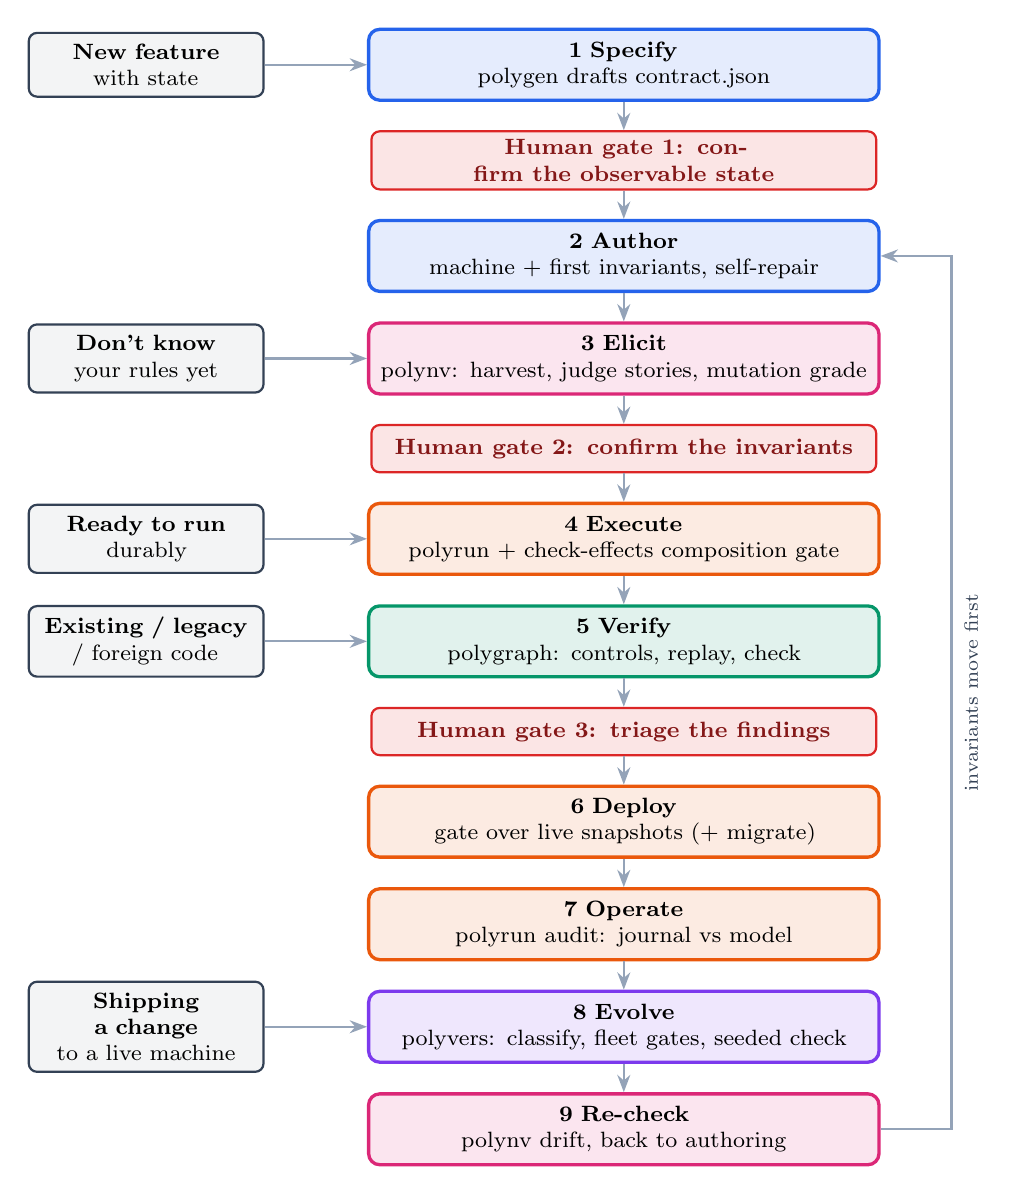
\begin{tikzpicture}[node distance=3.6mm and 13mm]
\node[phase=cGen] (p1) {\textbf{1 Specify}\\ polygen drafts contract.json};
\node[gate, below=of p1] (g1) {Human gate 1: confirm the observable state};
\node[phase=cGen, below=of g1] (p2) {\textbf{2 Author}\\ machine + first invariants, self-repair};
\node[phase=cNv, below=of p2] (nv) {\textbf{3 Elicit}\\ polynv: harvest, judge stories, mutation grade};
\node[gate, below=of nv] (g2) {Human gate 2: confirm the invariants};
\node[phase=cRun, below=of g2] (p3) {\textbf{4 Execute}\\ polyrun + check-effects composition gate};
\node[phase=cGraph, below=of p3] (p4) {\textbf{5 Verify}\\ polygraph: controls, replay, check};
\node[gate, below=of p4] (g3) {Human gate 3: triage the findings};
\node[phase=cRun, below=of g3] (p5) {\textbf{6 Deploy}\\ gate over live snapshots (+ migrate)};
\node[phase=cRun, below=of p5] (p6) {\textbf{7 Operate}\\ polyrun audit: journal vs model};
\node[phase=cVers, below=of p6] (p7) {\textbf{8 Evolve}\\ polyvers: classify, fleet gates, seeded check};
\node[phase=cNv, below=of p7] (nvd) {\textbf{9 Re-check}\\ polynv drift, back to authoring};

\foreach \a/\b in {p1/g1,g1/p2,p2/nv,nv/g2,g2/p3,p3/p4,p4/g3,g3/p5,p5/p6,p6/p7,p7/nvd}
  \draw[flow] (\a) -- (\b);

\node[door, left=of p1] (d1) {\textbf{New feature}\\ with state};
\node[door, left=of nv] (d2) {\textbf{Don't know}\\ your rules yet};
\node[door, left=of p3] (d3) {\textbf{Ready to run}\\ durably};
\node[door, left=of p4] (d4) {\textbf{Existing / legacy}\\ / foreign code};
\node[door, left=of p7] (d5) {\textbf{Shipping a change}\\ to a live machine};
\foreach \d/\t in {d1/p1,d2/nv,d3/p3,d4/p4,d5/p7}
  \draw[flow] (\d) -- (\t);

\draw[flow] (nvd.east) -- ++(0.9,0) |- (p2.east);
\node[rotate=90, font=\scriptsize, text=cInk] at ($(p2.east)!0.5!(nvd.east)+(1.15,0)$) {invariants move first};
\end{tikzpicture}
\caption{The \tool{polygraph} lifecycle. Five entry doors on the left feed a
spine of nine phases across the five engines; the three human gates (in red) are
the only points where a person is required. Evolution loops back to authoring
under the rule that invariants move first.}
\label{fig:sdlc}
\end{figure}

\subsection{\tool{polygen}: authoring checkable code}

\tool{polygen} authors new machines so that they are verifiable from the moment
they are written. From a paragraph of intent, it drafts the
\code{contract.json}, and here the first human gate falls: a person confirms
that the contract scopes the right observable state. \tool{polygen} then
authors the SAM v2 module, proposes an initial \code{invariants.mjs},
model-checks its own output against those invariants, and when it finds a
violation it repairs the code, never the invariants, because an invariant
encodes intent by definition and a disagreement between code and invariant
means the code is wrong. It cross-checks the vocabulary of the contract against
that of the code and synthesizes a replayed regression corpus. A run that did
not converge says so; the report never presents partial verification as clean.

\subsection{\tool{polynv}: eliciting the invariants}

The second human gate, confirming the invariants, was historically the hard
one, because writing predicates from a blank page is a scarce skill. The fifth
engine exists to make that gate cheap. \tool{polynv} turns invariant authoring
into invariant judgment. It harvests candidate rules mechanically, some mined
from the fleet and the execution journal against a grammar of property
templates, some proposed from domain priors, and pre-checks each one. It then
presents each candidate not as a predicate to write but as a concrete situation
to judge: the machine can reach this state today, here is the shortest path to
it, is that acceptable? Rejecting the story confirms an invariant with its
counterexample already attached. This design follows a robust finding from the
requirements-engineering and specification-mining literature, that people
cannot reliably enumerate their invariants but can judge concrete scenarios
instantly~\cite{daikon, vanlamsweerde}.

\begin{example}[Example: eliciting a rule by judging a story]
Asked ``what are your invariants,'' a designer of an order machine offers
generalities. Shown a specific reachable state instead, the answer is immediate.
\tool{polynv} presents: ``the machine can reach an order that is
\code{refunded} with \code{shipped = true}; here is the four-step path that
reaches it; is this allowed?'' The designer answers ``no.'' That single judgment
is an invariant, \code{not(refunded and shipped)}, now written down with its
counterexample attached, its author recorded, and its consequences, the other
states it forbids, shown back for confirmation. The designer authored a formal
rule without writing a predicate.
\end{example}

\tool{polynv} then grades the resulting invariant set by mutation. It
mechanically perturbs the machine, negating a guard, retargeting a transition,
freezing a field, and checks whether the invariant set catches the change. A
surviving mutant is a hole, shown concretely: the machine was broken in this
specific way and no rule noticed, what rule should have caught it? Because the
machine has a finite declared state graph, the notorious equivalent-mutant
problem, undecidable in general, is here decidable by comparing the state
graphs of the original and the mutant, so behaviorally equivalent mutants are
discarded mechanically and the grade is meaningful. The grade is disclosed in
the compatibility report as a trust tier, so a clean verification against a
weak invariant set cannot masquerade as a strong one. This mutation-based
assessment of oracle strength is itself an established technique~\cite{oracle,
specfuzzer}; the contribution here is applying it to intent, and making it
decidable via the finite domain.

Independent and recent work corroborates both the need for this gate and the
choice of mechanism. TLA-Prover, a system that fine-tunes a model to synthesize
TLA+ specifications, grades each output into four tiers and makes the top tier,
which it calls Diamond, a mutation-sensitivity check: the invariant is perturbed
at the syntax level and the model checker must then find a
counterexample~\cite{tlaprover}. Its stated purpose is exactly \tool{polynv}'s,
to deny credit for trivial invariants such as a tautology that passes the checker
while asserting nothing. Two independent groups converging on
mutation-sensitivity as the defense against vacuous verification is stronger
evidence for the principle than either could provide alone. The convergence also
sharpens where the two differ: TLA-Prover mutates the invariant's abstract
syntax, whereas \tool{polynv} mutates the machine and compares finite state
graphs, which lets it discard behaviorally equivalent mutants that a purely
syntactic mutation cannot recognize.

Two design rules protect the gate. Harvested candidates are behavior, not
intent: nothing enters \code{invariants.mjs} without an explicit, attributed
human disposition. And the interview is never delegated to the agent; the
engine prepares the questions and grades the answers, but the dispositions
belong to the person. To guard against an agent-led dialog drifting into mutual
agreement, every accepted rule is immediately run against the corpus and the
model check, and the dialog leads with the consequences, so the conversation is
anchored to executable evidence rather than to assent.

\subsection{\tool{polyrun}: executing durably}

\tool{polyrun} executes verified machines durably, in the manner of a
durable-execution engine, but with one architectural choice that matters for
everything downstream. Durability is snapshot-based rather than replay-based.
Rehydrating an instance is a matter of initializing the module and setting its
state from the stored snapshot, so there is no requirement that workflow code
remain deterministic with respect to every history it might replay, and
therefore no permanent versioning tax on future changes. Each step commits in
one transaction, the journal row, the snapshot, the effect intents, and the
timers together or not at all, and effects are emitted exactly once and
executed at least once under idempotency keys. A composition gate,
\code{check-effects}, explores the machine composed with its effect mapper
against emission invariants such as ``no path emits the charge effect twice''
and ``spawns exactly the declared number of children, and never before a
successful charge,'' which closes the double-charge class before deployment
rather than after. The execution journal is, by construction, the trace corpus
that the audit and the versioning gates consume.

\subsection{\tool{polygraph}: verifying against reality}

\tool{polygraph} audits stateful code that already exists, in any language,
against an independent reading of that code. It generates several specifications
of the code, independently, and replays each against traces captured from the
real system, then model-checks the surviving specification against the
invariants. Two disciplines make the audit trustworthy. Controls come before
trust: a hand-written correct specification must replay perfectly and a
deliberately mutated one must fail, proving the harness can tell good from bad
before any generated specification is believed. And the replay finds
unfaithfulness while the model check finds bugs: a faithful specification
reproduces the code's own bugs, so replay alone cannot see them, and it is the
exhaustive exploration against intent invariants that surfaces the reachable
bad state with a shortest path to it as a ready reproduction. Here the third
human gate falls: a person triages the findings, because a finding is a lead to
investigate, not a verdict to accept, and a finding against a reference or
third-party system may be an intent observation rather than a defect.

\subsection{The three human gates}

The lifecycle has exactly three points where a human is required, and they
correspond precisely to the two decisions no machine can make plus the one
judgment that closes the loop. Gate one confirms the observable state, the
contract. Gate two confirms the invariants, the intent. Gate three triages the
findings. What an agent must never do alone, and what teams should encode as a
norm, is approve a contract, approve an invariant, disposition an elicitation
question, dismiss a finding, or weaken a rule to make a check pass. Those
refusals are the whole of the human job. Measured in hours it is small.
Measured in consequence it is decisive, because every guarantee the toolset
offers is relative to those human decisions.

\section{\tool{polyvers}: compatibility checking for evolving state machines}

\tool{polyvers} is the engine we regard as novel, and this section treats it in
detail. It makes the compatibility question executable: given two versions of a
machine's artifact family and a source of live state, it classifies the change,
runs exactly the checks the change requires, and emits a compatibility report
that a deployment can be gated on. The design of the engine grew out of an
extended analysis of why versioning a state machine is hard and what a correct
answer would have to check, and this section carries the substance of that
analysis, because it is the foundation of the approach.

\subsection{The industrial default: reconstruction is not safety}

It is worth stating clearly what the dominant industrial answer does, because
\tool{polyvers} is defined largely by what that answer leaves unchecked, and it
is worth stating against the current mechanism rather than a deprecated one.
Event-sourced replay engines, of which Temporal is the most refined,
reconstruct the state of a running workflow by re-executing its code against a
recorded history of events. This has a genuine virtue: the history is a perfect
audit of past decisions, and it enables debugging by full deterministic replay,
which the snapshot model gives up. The classic cost was that workflow code had
to remain deterministic with respect to every history it might ever replay, so
behavioral changes were wrapped in versioned branches (the \code{patched} and
\code{getVersion} idioms) that littered the code and had to be kept alive until
the last old execution drained.

Temporal has moved past the worst of that. Worker Versioning with Build IDs now
lets a team pin a workflow type to the worker version it started on and route
only new executions to new code, draining old executions on old workers, and
Upgrade-on-Continue-as-New removes the need to patch for many long-running
patterns~\cite{temporalwv}. A reviewer from this world will rightly ask why not
simply pin the build and drain. The answer is the heart of this paper, and it
survives the newer mechanism intact. Build IDs solve \emph{routing}: which
worker version runs which execution. They do not solve \emph{safety}: whether
the new logic is correct for the state the old version will leave behind when an
execution does move forward. Pinning and draining postpone the compatibility
question and, for auto-upgraded or continued executions, still hand old state to
new code with no invariant check. Draining guarantees that old state can be
reconstructed and finished on old logic; it never checks that new logic is safe
for old state. The distinction between reconstruction and safety is exactly what
\tool{polyvers} targets, and it is orthogonal to how executions are routed.

The deeper point is what all of that discipline actually guarantees. It
guarantees that old state can be \emph{reconstructed}. It does not guarantee
that the new logic is \emph{safe} for that state. Those are different questions,
and replay answers only the first. A workflow can replay its history perfectly
and then take its next step, under the new code, straight into a state its
invariants forbid. The reconstruction was flawless and the outcome is still
wrong. \tool{polyvers} is built to answer the question replay does not ask: not
``can I rebuild the old state,'' but ``is the new machine safe for the old
state that already exists.'' Everything that follows is a decomposition of that
question into checkable pieces.

\subsection{Refusing to treat ``compatible'' as one question}

The core move is to refuse the single question ``is the new version
compatible?'' and to replace it with a small number of separately checkable
questions, one per kind of change. A content-hashed difference of the artifact
family fires \emph{lanes}. The shape lane fires when the declared state keys
change. The vocabulary lane fires when the actions, reject reasons, effect
kinds, or terminal states change. The intent lane fires when the invariants
change. The semantic lane fires when the module changes with the same shape and
vocabulary. The migration lane fires when a migration function is added or
edited. The composition lane fires when the effect mapper changes. Each lane
names exactly the gates it demands, and a cosmetic edit fires no lane at all,
and the report says so. This decomposition is itself a contribution, because
the industry routinely conflates these and thereby misjudges which changes are
dangerous.

Three of the lanes carry a distinct insight worth stating on its own. The shape
lane asks a question replay never poses. Because the SAM v2 strict profile makes
the observable state a sealed declaration that round-trips totally, shape
compatibility stops being a matter of code review and becomes a mechanical test:
take every live production snapshot, round-trip it through the new module, and
compare canonically. A snapshot the new machine mangles or rejects fails the gate
before any instance sees the new code. This is precisely the check replay does
not give, because replay asks ``can I rebuild this state,'' which is a different
and weaker question than ``does the new machine accept this state.'' The
vocabulary lane converts drift into a boot-time error rather than a runtime
surprise weeks later: because actions, effect completions, and spawn wirings are
all declared, a completion wired to an action the machine no longer exports, or a
parent spawning a child whose cancel action has disappeared, is caught at
registration. Renaming an action is therefore loud by construction, and the
failure mode of vocabulary drift is a refused boot, which is the correct failure
mode. The intent lane rests on a single rule of order, that invariants move
first. Strengthening an invariant is a compatibility event against a machine's
own fleet, and the gate names the live instances that already violate the
stronger rule; weakening one is a decision that deserves a diff in review rather
than an accident of code drift. Because the invariants are a small standalone
artifact, their history is the semantic changelog of the system, something no
amount of reading code diffs reconstructs reliably.

\subsection{The headline: fleet-seeded model checking}\label{sub:seeded}

The semantic and intent lanes carry the central idea. Define the observable
state that production actually holds as the \emph{fleet}. The strongest gate
re-runs the exhaustive bounded exploration, but instead of starting only from
the machine's initial state, it seeds the exploration with the live fleet
snapshots as additional initial states. The question it answers is not ``is the
new machine correct from its initial state,'' which is the ordinary
model-checking question, but ``can any state that a live instance currently
holds be driven, under the new rules, to a state that violates the
invariants.''

This yields a precise definition of semantic compatibility that the field has
lacked: version $n{+}1$ is semantically compatible with the fleet of version
$n$ if and only if every live state of version $n$ satisfies the invariants and
cannot be driven to a violation under the transition function of version
$n{+}1$, over the declared finite domains. This is a computable property, not a
review checkbox. It is exactly the landmine hunt mechanized, because the checker
does not care whether the new version could have constructed a given state; it
cares what the new version will do with the state that already exists.

\begin{example}[Example: a landmine that only the seeded check finds]
Version one of an order machine allows an order to be refunded while a shipment
is still in flight, so production holds instances with
\code{status = refunded} and \code{shipping = active}. Version two removes the
transition that produced that combination and strengthens the rules so a
refunded order should never ship. A test suite for version two will never
construct the forbidden combination, because version two cannot reach it from
its own initial state, and a shape or vocabulary diff sees nothing wrong: the
keys and actions are unchanged. Yet the combination sits in the live fleet.
Seeded with that snapshot, the exhaustive check fires the delivery action, drives
the instance into \code{status = refunded, delivered = true}, and reports a
violation with the shortest path from the seed as the reproduction. The same
change passes every check that does not start from the state production actually
holds.
\end{example}

Figure~\ref{fig:seed} contrasts the ordinary model check, which starts only from
the machine's initial state, with the seeded check, which adds the live fleet
snapshots as additional starting points.

\begin{figure}[t]
\centering
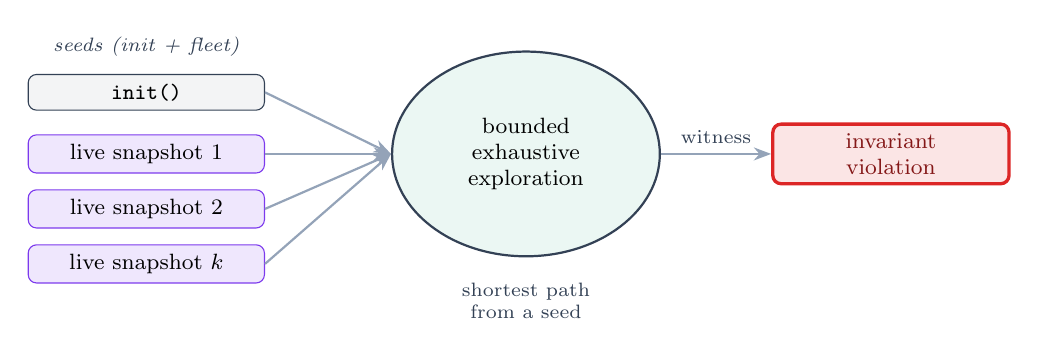
\begin{tikzpicture}[font=\footnotesize]
% seeds column
\node[rectangle, rounded corners=3pt, draw=cInk, fill=cInk!6, minimum width=30mm, align=center] (init) {\code{init()}};
\node[rectangle, rounded corners=3pt, draw=cVers, fill=cVers!12, below=3mm of init, minimum width=30mm, align=center] (s1) {live snapshot 1};
\node[rectangle, rounded corners=3pt, draw=cVers, fill=cVers!12, below=2mm of s1, minimum width=30mm, align=center] (s2) {live snapshot 2};
\node[rectangle, rounded corners=3pt, draw=cVers, fill=cVers!12, below=2mm of s2, minimum width=30mm, align=center] (s3) {live snapshot $k$};
\node[font=\scriptsize\itshape, text=cInk, above=1mm of init] {seeds (init + fleet)};
% exploration
\node[ellipse, draw=cInk, thick, fill=cGraph!8, right=16mm of s1, minimum width=34mm, minimum height=26mm, align=center] (bfs) {bounded\\ exhaustive\\ exploration};
% violation
\node[rectangle, rounded corners=3pt, draw=cGate, very thick, fill=cGate!12, right=14mm of bfs, text=cGate!60!black, align=center, minimum width=30mm] (v) {invariant\\ violation};
\draw[flow] (init.east) -- (bfs.west);
\draw[flow] (s1.east) -- (bfs.west);
\draw[flow] (s2.east) -- (bfs.west);
\draw[flow] (s3.east) -- (bfs.west);
\draw[flow] (bfs.east) -- (v.west) node[midway, above, font=\scriptsize, text=cInk]{witness};
\node[font=\scriptsize, text=cInk, below=2mm of bfs, align=center] {shortest path\\ from a seed};
\end{tikzpicture}
\caption{Fleet-seeded model checking. The ordinary check explores only from
\code{init()}; \tool{polyvers} additionally seeds the exploration with the states
the live fleet holds, so a violation reachable only from a currently existing
state is found, with the shortest path from a seed as the witness.}
\label{fig:seed}
\end{figure}

The implementation is disciplined about what the seeding means. Seeds are
exempt from the exploration cap, because the cap bounds what exploration
discovers, not how many snapshots the fleet already holds; otherwise a fleet at
or above the cap would report a bounded result with zero transitions tried. A
failing verdict names one witness per violated rule, the shortest path from a
seed to the violation, and the report is explicit that this is a compatibility
verdict rather than the full list of affected instances. And the provenance of
the corpus is part of the verdict: archived fleet state is the honest tier,
while synthesized states, the states the old model says are reachable, are the
weakest tier, disclosed as such, precisely because a landmine violates the
assumption that the old model's reachable set covers what production holds.

Three technical points determine whether the gate is tractable and honest in
practice. First, the quantity that matters is not the size of the fleet but the
number of \emph{distinct} observable states it holds. A million instances
typically collapse to a small set of canonical snapshots once projected to the
observable state, because most instances are in one of a few situations, so the
seed set is usually small even for a large fleet, and deduplication by canonical
form makes this automatic. Second, and less comfortably, running is not passing.
For the gate to pass rather than merely run, the exploration forward from every
seed must terminate within the exploration cap without hitting it; a run that
hits the cap is reported as bounded, which is a failing verdict. On a large
declared domain this completeness threshold is a real operational question, and
a gate that is honest but frequently fails bounded is very different from one
that passes cleanly. We report the behavior on the worked example below and name
honest scaling as future work rather than claiming it. Third, a fleet seed is a
state, not a pending transition, so transition-level invariants are checked only
on the transitions the exploration generates forward from a seed, and never on
the transition that happened to be in flight when the snapshot was taken; state
invariants are checked on the seed itself. Callers who encode a safety property
as a transition invariant should know it is evaluated over forward steps from
the fleet, not over the interrupted step.

An empty corpus is refused for a version deployment, never treated as a vacuous
pass, but the greenfield case is different and the tool distinguishes it: the
first deployment of a machine that has no production instances has a legitimately
empty fleet, and there the empty corpus is a pass with the model check run from
\code{init()} alone, not a refusal. The refusal applies to a change deployed
against a fleet that should exist but was not supplied, which is the case where an
empty corpus would silently verify nothing.

\begin{table}[t]
\centering
\small
\begin{tabular}{@{}p{4.4cm}p{2.3cm}p{6.2cm}@{}}
\toprule
\textbf{The change} & \textbf{Lane} & \textbf{The checks that gate it} \\
\midrule
Same shape and vocabulary, new transition rules &
Semantic &
Strict validate; round-trip over live snapshots; invariants pointwise; model
check seeded from live states \\[0.4em]
Declared state keys change &
Shape / migration &
The above over the migrated states; projection equality; two-phase, fenced,
journaled apply \\[0.4em]
Actions, reject reasons, or completions change &
Vocabulary &
Domain cross-checks; manifest wiring checks at load; stale-stimulus rejection
across the window \\[0.4em]
Invariants change &
Intent &
Invariant diff; pointwise re-check on the live fleet; seeded model check for
reachable violations \\[0.4em]
Effect mapper changes &
Composition &
\code{check-effects} path exploration: emissions, spawn counts, timer validity \\
\bottomrule
\end{tabular}
\caption{The compatibility lanes as a decision table. A cosmetic edit fires no
lane, and the report says so.}
\label{tab:lanes}
\end{table}

Table~\ref{tab:lanes} summarizes the lanes as a decision table over the kind of
change, which is how \tool{polyvers} presents its classification before running
any gate.

\subsection{Cross-version delivery, and one unification}

Time does not stop for a deployment. A timer armed by version one fires into
version two. An effect completion requested by version one arrives at version
two. \tool{polyvers} checks this by the same doctrine the toolset uses for
at-least-once delivery within a single version: observable rejection. Every
stimulus the old version could still deliver is fired at the new machine in
every fleet state, and each outcome must be accepted or a named observable
reject; an unhandled stimulus, a throw, or an unnamed reject fails the gate. The
deep point is a unification: a machine that is verified safe under redelivery is
safe under cross-version delivery, because the two are the same problem, and the
toolset solves it once at the verification layer rather than twice at the
infrastructure layer.

One qualification belongs here rather than only in the threats section, because
it is easy to over-read the unification. The two problems coincide on the
\emph{safety} question but not on the \emph{liveness} one. Proving that version
two safely rejects a stale version-one stimulus proves that nothing bad happens;
it does not prove that the right thing happens. A version-one timer that version
two safely rejects may have been the very timer that was supposed to advance the
instance, and the instance is now safely stuck. The gate is a safety gate, so a
change that silently stops doing something a safety invariant never required will
pass it (see Section~8). Observable rejection makes cross-version delivery safe;
it does not make it live, and a team relying on a stimulus to make progress must
state that as a property the safety gate cannot see.

\subsection{Migration as a gated, fenced, journaled artifact}

When the shape genuinely must change, the migration function receives the same
treatment as any other artifact, because it is one. It is pure, a function from
old state to new state with no input or output and no clock, which makes it
checkable. \tool{polyvers} scaffolds it from the shape difference, complete for
pure additions and with explicit unfilled holes for the rest, and the migrate
gate validates it across the whole fleet: the new module accepts every migrated
snapshot, the result equals the module's own observable projection so that stray
keys cannot poison later steps, and the invariants hold on every migrated state.
Validation is two-phase, validating everything before applying anything, so a
fleet is never left half-migrated by one instance's unusual state. Application
is fenced on the sequence number observed at validation time, so an instance
that took a live step in between is skipped and reported rather than overwritten.
And each applied migration writes a journal row recording the old and new
snapshots, stamped with the new version, so the audit trail survives the
migration rather than being broken by it. A validated migration then swaps the
corpus, so that every downstream gate runs over the states the fleet will hold
after the migration.

This lane is best understood as \emph{state upcasting} in the sense the
event-sourcing community has developed for schema evolution, where an upcaster
transforms stored data of an old shape into the new shape and the rest of the
system sees only the latest version~\cite{upcasting}. The migration lane is a
snapshot upcaster with two additions the event-sourcing practice does not
usually make mechanical: it is validated across the whole fleet against the new
module's own acceptance and the invariants before any instance is touched, and
it is applied under a fence on the sequence number observed at validation time.
Situating it this way is deliberate: the migration lane's nearest neighbor is
schema-evolution and upcasting work, not behavioral subtyping, and the
contribution is the fleet-wide validation and fencing rather than the
transformation itself.

\subsection{The observable-state projection is the ceiling}\label{sub:projection}

The single most important limitation of \tool{polyvers} is not a bounded
exploration or a missing feature; it is a property of the whole approach, and it
deserves to be stated as plainly as the central idea. Every guarantee the engine
offers is relative to the observable-state projection declared in
\code{contract.json}. The seeded check is only as complete as that projection is
faithful. If real coupling that determines reachability lives outside the sealed
snapshot, then a fleet of observable snapshots does not capture the state that
actually governs what the machine can do, and the exploration can report clean
while a genuine landmine sits in the un-modeled dimension. Armed timers,
in-flight effect state, external dependencies, and correlations across instances
are exactly the kinds of coupling that a per-instance observable projection can
omit. State outside the projection is not checked, not migrated, and not
audited, by construction.

This limitation is not hypothetical, and the fleet study of
Section~\ref{sub:fleetstudy} priced it. Replaying a real released change, the
engine missed a genuine behavioral difference affecting zero-amount records
because the money abstraction the contract declared has three values and
collapses when the total is zero. The state that mattered was not outside the
projection by oversight; it was outside by a declared abstraction that had been
committed before the analysis ran. The guarantee held exactly as advertised, over
exactly the state the contract named, and a real defect lived in the gap. We
consider this the most useful evidence in the study, because a ceiling that is
only ever conceded in the abstract is not a ceiling a reader can calibrate
against.

This reframes an item that an earlier version of this paper listed separately.
The cross-machine joint-state gap of Section~\ref{sub:product} is not a distinct open problem;
it is this same limitation showing its edge. A parent and a child are coupled
through a joint state that no single machine's observable projection contains, so
until that joint state is itself made observable and seeded, the product check
inherits exactly the projection ceiling described here. The honest way to read
the whole engine is that it verifies compatibility over the state a team chose to
make observable, and that choosing the projection well is therefore the real
skill the approach demands, the analog at the versioning layer of choosing the
invariants well at the authoring layer.

\subsection{Sagas, compensation, and what the effect gate does not check}

The running examples in this paper, the double charge and the refund after ship,
are saga-shaped, and honesty requires saying precisely what the machinery does
and does not check about them, because it is easy to promise more than is
delivered. The composition gate, \code{check-effects}, reasons about emission
invariants: how many times an effect is emitted, in what state, and in what
order relative to the machine's own transitions. It establishes properties like
``no path emits the charge effect twice'' and ``a shipment is never spawned
before a successful charge.'' What it does not currently reason about is
compensation correctness: when a refund follows a shipment, whether the
compensation logic correctly unwinds the charge, the inventory hold, and the
shipment, in the right order, idempotently. Those are the hard bugs in this exact
domain, and they live in the effect handlers, which are the part of the system
whose correctness is the developer's responsibility rather than the checker's.

We therefore scope the claim rather than overstate it. Where a compensation can
be expressed as a transition of the machine itself, so that the unwinding is a
sequence of actions over the observable state, it falls inside the semantic and
composition gates like any other behavior. Where a compensation is logic inside
an effect handler, coordinating several external systems, it is outside the
model, and the toolset checks only that the handler is invoked with the right
idempotency key on the right transition, not that its rollback is semantically
correct. A compensation-invariant language over the effect mapper, able to state
``every emitted charge has a matching refund on the compensating path,'' is a
natural extension and is recorded as future work; it does not exist today, and
the examples should be read with that boundary in mind.

\subsection{Deployment: the gate verdict, and the escape valve}

A natural objection is that a gate which refuses any version that cannot accept
the live fleet is too blunt for production, where there is always a strange
instance somewhere: a stuck order from a bug three quarters ago, a hand-edited
row. If a single non-conforming snapshot blocked every deployment, that would be
a serious operational constraint that the replay-and-drain model does not impose,
since it ships new-execution code immediately and lets stragglers finish lazily.
The honest position has two parts. The compatibility \emph{verdict} is indeed a
property of the corpus: one snapshot that the new rules can drive to a violation
fails the semantic gate, because a clean verdict over a corpus that contains a
landmine would be false. But the \emph{deployment} is not all-or-nothing, because
the toolset separates the outliers from the verdict by two existing mechanisms.
The migrate apply is fenced per instance, so an instance that cannot be migrated
cleanly, or that moved during the apply, is skipped and reported rather than
forced. And the poison doctrine is exactly a quarantine: an instance for which
something that cannot happen has happened is durably set aside, loudly, and
excluded from the live set, so the operational pattern the objection asks for,
quarantine the outliers, ship, and resolve them asynchronously, is supported by
cohorting the fleet, gating and shipping the conforming cohort, and carrying the
quarantined outliers as named, tracked exceptions rather than as silent blockers.
What the toolset deliberately does not offer is a way to ship a version over a
fleet that contains an un-quarantined landmine while calling the result clean.
The escape valve is explicit quarantine, not a suppressed verdict.

\subsection{The honest ledger, and the version-aware audit}

Honesty requires the other column of the ledger, because the snapshot approach
gives up something replay provides for free. Event-sourced history is a complete
record of which decisions were made by which code, reconstructible at any point.
The toolset earns that guarantee back piecewise rather than getting it whole. The
execution journal records the machine version of every step, migrations leave
explicit records carrying both the old and the new state, and the trace corpus
for each version can be replayed against that version's own specification. This
is a reconstruction of the same guarantee at the level of observable behavior
rather than at the level of the executed decision procedure, which is enough for
most purposes and costs no determinism sandbox; but a compliance regime that
must replay the literal decision procedure of eighteen months ago is a case where
event sourcing still holds a card the snapshot model does not.

This version-aware journaling pays off directly in the continuous audit.
Because each window records the version that produced it, windows journaled
under an older machine version are counted and reported rather than replayed
through the current module, so a shape migration does not convert an entire
pre-migration history into false drift, while a genuine divergence, a hot patch
or a manual edit to the database, still surfaces. In most systems a migration is
precisely the moment the history stops being checkable; here it is a recorded
event in an audit trail that survives it.

There is one more honest trade to name. Replay makes it possible, if painful, for
a single worker to serve arbitrarily old in-flight executions indefinitely. The
snapshot model instead forces the compatibility question at deploy time: a
version that cannot accept the live fleet may not ship. We regard forcing the
question early as the feature rather than the defect, but it is a real constraint,
and a team that habitually lets years-old executions drift will find itself in
the migration lane more often as a result.

\subsection{The cross-machine product, and what remains open}\label{sub:product}

Orchestration adds a dimension: a parent machine of version two may drive a
child machine of version one during a rollout. \tool{polyvers} checks the
protocol and delivery of every parent-old-or-new by child-old-or-new pairing,
and, in its most recent form, checks the joint product of the two machines
against cross-machine invariants for each pairing. The fixture that proves the
value is a child whose cancel window narrowed between versions: it passes the
protocol and delivery matrix, because the cancel still lands as a named reject,
and fails the product check, because the shipment delivers under a cancelled
order.

Honesty about the open edge is part of the design. The joint product is
currently explored from the initial pairings, not seeded from the live joint
state of the fleet, because that requires a joint export of parent and child
snapshots that is recorded as future work. The single-machine landmine argument
applies identically to the joint state space, so until the real interleavings of
the fleet seed the product check, the joint gate is exhaustive from the initial
state rather than from reality. This is the most important open item in the
engine, and it is stated in every report.

A second open item is different in kind, because it is not a gap in the tooling
but a decision the tooling deliberately refuses to automate. Call it meaning
migration. When the state space of the new version has no honest image for some
state of the old version, and the problem is not the shape of the data but its
meaning, no pure function can resolve it. There is no correct answer to ``what
does this instance become'' that a program could compute, because the question
is what those instances now mean, and that is a human judgment. The gate's
contribution is not to answer the question but to make it arrive at the right
time. It fails loudly, before the deployment, attached to a named list of the
affected instances, so that a person decides what they mean while there is still
a decision to make, rather than after the deployment, attached to an incident
page.

\subsection{A worked example, with numbers}

The concrete example that accompanies the engine is an order-management
machine. Version one is a single order state machine with a charging step and a
fulfillment rollup; version two changes the shape by adding a key, changes some
transition rules, and strengthens an invariant, all at once, which is the case
that most versioning schemes handle worst because several kinds of ``version''
change together. On this change the classifier fires the shape, migration,
intent, and semantic lanes and names the gates each requires. The committed
compatibility report gives concrete numbers, which we report here precisely
because the paper is otherwise a design paper. The corpus was thirty-three
snapshots, and its provenance is stated in the report as synthesized, the
BFS-reachable states of the old machine, which the report explicitly labels the
weakest tier and recommends replacing with live or archived snapshots. Those
thirty-three snapshots were migrated through the new version's migration function
before the downstream gates ran. The migration validated over all thirty-three
(pure, accepted, projection-equal, with state and transition invariants holding).
The pointwise gate ran four state invariants over thirty-three snapshots, which
is one hundred thirty-two checks. The seeded semantic model check ran from the
thirty-three fleet snapshots plus \code{init()} and discovered seven states, and
it passed cleanly rather than bounded. The invariant adequacy line reads NOT
MEASURED, disclosing that the strength of the invariant set was not graded in
this run, so a passing verdict is weaker than it looks until \tool{polynv}'s
mutation grade is applied. The parent-by-child rollout matrix then checks the
version pairings of the order machine against its shipment child.

Two things about these numbers are worth stating plainly. The first is that they
demonstrate the mechanism firing end to end and, just as importantly, the
report's honesty machinery working: the corpus tier and the ungraded adequacy are
disclosed as part of the verdict rather than hidden behind a green checkmark. The
second is what they are not. This is a worked example on synthesized states, not
a production fleet, and it cannot on its own say how many landmines the gate
catches that a team's existing process would have missed. That question required
a separate study, which we now report.

\subsection{The fleet study}\label{sub:fleetstudy}

An earlier version of this paper listed a real-fleet case study as future work.
It has since been carried out, pre-registered, in three tiers of increasing
independence: a fixture matrix that varies corpus provenance while holding the
change fixed; a subscription-billing fleet modeled on a public payments API; and
an archaeology tier that replays released version pairs of Medusa, an
open-source commerce backend, and scores against the maintainers' own record.
The pre-registration, the case taxonomy, the null results, and the run harness
are committed in the repository under \code{eval/fleet-study/}~\cite{repo}. Two
methodological points govern how the numbers below should be read. First, the
study is a controlled test of the mechanism and of the effect of corpus
provenance; it is not an estimate of a true-positive rate, and the harness
deliberately refuses to compute rate statistics over corpora the models under
study generated. The reader should therefore weigh the results as existence and
controlled-contrast findings, not as performance metrics. Second, the discipline
that every number depends on is a freeze: in the archaeology tier the model of
the old version is authored and committed \emph{before} the new version's diff is
read, so a finding cannot be an artifact of having known the answer. The freeze
commits are cited with the results (for the two Medusa pairs, the old-version
translations were frozen at \code{0f34c26} and \code{a305507} respectively,
before the corresponding v2.5.0 and v2.17.2 sources were read). The projects and
version pairs were selected independently of the analysis, on the availability of
released pairs and commit history rather than on any expected outcome; the
modeling, not the target selection, is what the freeze protects.

\paragraph{Provenance is the whole difference.} The first tier runs four
incompatible changes and two compatible ones against corpora that differ only in
where the states came from. On an archived corpus all four incompatible changes
are caught. On a synthesized corpus, the BFS-reachable states of the old machine,
only three of the four are caught. The one that escapes is the landmine: a state
that the old version could reach, that production therefore holds, and that the
new version's rules forbid. A synthesized corpus cannot contain it, because it
contains only states the old \emph{model} says are reachable. The same tool, the
same change, and the same gates report a pass or a failure depending on nothing
but corpus provenance. Both compatible changes stay clean on both tiers, so the
tier reports no false positives. The composition cases in the same tier separate
the two levels of the cross-machine check: a narrowed cancellation window passes
the pairwise version matrix and fails the joint product check, which is the
concrete form of the gap Section~\ref{sub:product} declares open.

\paragraph{A machine can be internally consistent and still unsafe to deploy.}
The second tier builds a subscription-billing machine after a public payments
API and ages a fleet of four hundred subscriptions, cutting each trajectory at a
seeded point so that records are caught mid-flight rather than settled; that one
change took the corpus from three distinct states to eleven and was forced by
looking at the first capture rather than by theory. The collapse of four hundred
instances to eleven distinct states is the tractability point of
Section~\ref{sub:seeded} observed in the field: what the check seeds from is the
number of distinct canonical snapshots, not the raw fleet size. Three version changes are
then run against it. The interesting one narrows a dunning retry budget from
three to two and tightens the invariants with it. Checked from \code{init()} the
new version explores nineteen states and reports no reachable violation: it is
internally consistent, and every state it can reach from a fresh start obeys
every rule it declares. Seeded from the fleet it fails, because the fleet holds a
subscription sitting in \code{pastDue} at exactly the depth the narrowed budget
makes terminal. A second finding follows from the first, and we report the
dependency rather than counting them separately: from that same live state a
single payment failure drives the machine past its own new budget, but
remediating the first finding removes the seed and the second disappears with it.
The population is one snapshot. We say so, because the class of defect and the
size of the blast radius are different claims.

\paragraph{Two real changes that looked identical and were not.} The third tier
replays two released pairs of a commerce backend whose payment status machines
changed in the window studied. Their one-line summaries are near-identical: in
each, a status enumeration gains members. The outcomes are opposite. In the first
pair the status derivation itself changed, so that a fully captured payment
collection is \code{completed} where the old version left it \code{authorized};
the shipped migration widens a database constraint and rewrites no row, and six
of thirty-two fleet states are stranded permanently, since the recompute that
would fix them runs only on operations a settled collection never receives
again. In the second pair the module service is untouched by the change commit
entirely, the new member is one more value providers may report into paths that
already wrote provider values verbatim, and no fleet state is affected. We
classify the first as true-but-intended rather than a true positive, and the
criterion deserves to be stated precisely, because ``intended'' could mean two
things and only one of them holds here. It does not mean the change was safe: the
migration the maintainers shipped is a constraint widening that addresses nothing
the finding is about, and six fleet states are stranded permanently regardless of
anyone's intent. It means only that the maintainers were \emph{aware}, since the
pull request that introduced the change names this inconsistency class in its own
description as work still to do. Our pre-registered rule reserves ``true
positive'' for a finding that names a data migration the maintainers had to ship
and did not, and awareness disqualifies it under that rule, so we apply the weaker
label rather than stretch a pre-registered rule to flatter the result. We note,
however, that under a criterion keyed to safety rather than to awareness this
would be a true positive that the shipped migration failed to resolve, and a
reader who prefers that criterion should read it as one. The finding itself, six
permanently stranded states that the shipped migration does not reach, is not in
dispute either way.

The matrix is the finding here, more than either pair is. Two changes whose
human-legible summaries are interchangeable behave oppositely, and nothing short
of reading both diffs distinguishes them. A team classifying either change from
its release notes would have been wrong in both directions.

\paragraph{What it costs.} Every run in the study is local, deterministic, and
needs no API key; wall-clock times are seconds per change, and the per-run times
are recorded with the artifacts rather than estimated here. The real cost is
human and it falls in one place, which is where we think it belongs: writing the
migration. Both migrations in the second tier were scaffolded by the tool and
both needed a hand edit, for opposite reasons that are worth reporting together.
For a shape split the scaffold initialized a new key from the new contract's
initial state, which, applied as generated, would have migrated every
subscription in the fleet to a recurring amount of zero; the scaffold cannot
distinguish a rename from a new field, and only a human reading both contracts
can. For the narrowed budget the scaffold detected the domain narrowing and
\emph{refused to guess}, leaving a hole that throws. That refusal is the correct
behavior, because the question it declines to answer, what becomes of a record
sitting at a depth the new budget makes illegal, has several defensible answers
that are not equivalent, one of which silently hands an exhausted customer
another retry. The tool's contribution is not the conversion. It is that the
conversion became a reviewable artifact with a named hole instead of an implicit
assumption inside a deployment.

\paragraph{False positives, and one we caused ourselves.} Across both tiers the
engine raised no false alarm on a change that was in fact compatible. It did
raise one alarm we consider a taxonomy imprecision rather than a false one: a key
whose value domain was unchanged but whose \emph{role} changed was reported by
the shape lane rather than the semantic lane, and demanded a migration that no
data migration can address. Separately, and more instructively, our first run of
the archaeology tier reported four retyped keys of which two were noise we
introduced: the engine diffs a state key's declared type as a whole string, and
we had reworded two type descriptions without changing their meaning. That is an
operator error, not a tool defect, and we report it because a study that records
only the tool's mistakes is not measuring honestly, and because the distinction
between a tool crying wolf and an operator moving the goalposts is one a reader
cannot check unless it is written down.

\paragraph{What the study did not catch, and why.} The most useful single number
the study produced is a miss, and it falls squarely on the ceiling of
Section~\ref{sub:projection}. The clause the first archaeology pair adds tests
\emph{equality} between a captured amount and a total, so a zero-amount payment
collection satisfies it with nothing captured and no payment sessions at all: a
free order reads as unpaid under the old version and as completed under the new
one. Zero-amount collections are ordinary in commerce, arising from a full
discount or a gift card covering the total. The engine did not report this, and
the reason is legible in the contract rather than in the engine: the money
abstraction the model declares has three values, none, partial, and full, and it
\emph{collapses} when the total is zero, so the case is not expressible. That
abstraction bound was declared in the artifact before this analysis was done, not
added afterward to excuse the miss. We class it as out-of-projection rather than
as a limitation of the checking, and we regard it as the most valuable evidence
in the study, because it is the projection ceiling costing something measurable
on a real change instead of being conceded in the abstract.

\paragraph{What we still have not earned.} Three limits bound every number above.
The subscription fleet is generated rather than captured from a live account, and
because the generating machine is the one under study, a corpus produced that way
is circular as evidence about it; the harness therefore refuses to report
true-positive and false-positive rates over it, and that adjudication waits on a
live capture. The archaeology corpora are likewise derived from the frozen
old-version models rather than from a running instance of the application, which
is sound for the compatibility question actually asked, whether states the old
version declares legal remain legal under the new one, but is not evidence about
how faithfully the models track the application. And the archaeology tier
produced no true positive in the strict sense of a finding that names a data
migration the maintainers had to ship, because in the window we studied that
project shipped no such change: across two major versions its order and
fulfillment status machines never changed at all, and no released pair narrows a
state domain. That last observation is itself worth recording, and worth not
over-reading. It is evidence about what maintainers do, which is consistent with
narrowing being known to be expensive and avoided, and it is not evidence that
the problem is rare.

\subsection{Where this sits in the literature}

A survey of adjacent work places \tool{polyvers} in three neighborhoods, none
of which ships the combination. Behavioral subtyping and protocol
substitutability ask the same theoretical question, whether one version can
safely stand in for another, formalized as refinement between
automata~\cite{subtyping}. The catch is decidability: the question is tractable
for synchronous or regular interfaces but undecidable for asynchronous session
subtyping in general~\cite{session}, which is exactly why a bounded exploration
with an explicit cap, and a rule that a bounded result is not a pass, is the
honest posture rather than a limitation to apologize for. Verified dynamic
software updating asks the other half of the question, whether it is safe to
move a live instance from old to new and whether the state-transformation
function preserves correctness~\cite{dsu}, which maps almost one to one onto the
semantic gate plus the migrate gate; those are research prototypes on
constrained languages, hitting the same state-explosion wall. And what industry
deploys at scale is syntactic: schema and interface diffing, protocol
compatibility rules, semantic-versioning breaking-change detectors. These check
shapes and signatures, which are the toolset's shape and vocabulary lanes, and
never reason about reachable states or invariant preservation, which is exactly
the gap the landmine exploits.

The specific combination here, semantic compatibility of a state machine checked
not for all possible states, which is intractable, but for the finite set of
states the fleet actually holds, seeded into an exhaustive bounded exploration,
appears closer to bounded model checking over runtime state than to full
refinement checking, and we have not found published work framing it exactly
that way.

Two nearer neighbors deserve naming, because a reader will otherwise ask whether
this is just one of them. The first is directed or targeted model checking, which
explores from concrete states of interest rather than only from an initial
state~\cite{directed}; the seeded check is a directed check whose target states
are supplied by the live fleet, which is the specialization that makes it a
compatibility test rather than a general search. The second is the informal event-sourcing practice of replaying
production events against a rebuilt read model to see whether a new projection
behaves, which shares the instinct of checking new logic against real production
state but performs no forward exhaustive exploration and states no invariants over
reachable states. Neither does forward exhaustive exploration seeded from live
states for the specific purpose of version compatibility, so the combination
claim survives contact with both; naming them is meant to pre-empt the obvious
question rather than to hide behind it. The framing is therefore novel while
every ingredient has precedent, which is the honest and, we think, still valuable
claim. It is a literature claim about novelty; the separate empirical claim, that
the mechanism fires and that corpus provenance determines the verdict, is
supplied by the fleet study of Section~\ref{sub:fleetstudy}.

\section{Event-sourced replay and the gated snapshot approach}

Because event-sourced durable execution, of which Temporal is the leading
example, is the default against which this work is naturally compared, it
deserves a direct and fair treatment rather than a caricature. The comparison
also clarifies what the toolset is actually claiming, which is narrower and, we
think, sturdier than ``a better workflow engine.''

\subsection{Durability is a commodity; the differentiator is the gate}

It is tempting to frame the contrast as a kernel-versus-kernel contest, and that
framing is a mistake. The correctness core of durable execution, a transactional
outbox, idempotency keys, lease-based workers, and one commit per step, is a
well-understood problem with settled solutions. \tool{polyrun} delegates most of
it to a relational database, which means the trusted base for durability is
largely the decades of hardening in that database rather than any novel code.
Durability, in short, is close to a commodity. What a decade of engineering
genuinely bought Temporal is not durability but operational maturity at scale,
and this is worth stating without grudging, because it is real and the toolset
does not match it: sharded task routing and queue management across thousands of
workers, real-time visibility through a mature web console and CLI, multi-region
failover, and debugging by full deterministic replay of any execution. The
snapshot model gives up that last capability directly and earns only a weaker
version back piecewise, as Section~5 conceded. These are the properties a team
running millions of concurrent workflows depends on, and \tool{polyrun} does not
claim them.

The honest scoping is therefore explicit: \tool{polyrun} targets the median
durable-execution workload rather than the top of the scale, and the median
workload is a large market. We are careful not to over-assert the shape of that
distribution, which we have not measured; we claim only that a database-backed
engine comfortably covers workloads in the range of thousands of instances and
moderate event rates, which is where most stateful business software sits, and
that the minority of workloads requiring millions of concurrent executions with
multi-region failover is precisely the segment where Temporal's operational
investment is decisive. On the design axis, the field is visibly diversifying
away from full deterministic replay as the only recovery model: Restate records
completed operations in a per-invocation journal and replays that journal rather
than re-executing arbitrary code, and DBOS embeds durable execution as a library
that checkpoints workflow and step state into Postgres~\cite{restate, dbos}.
\tool{polyrun}'s snapshot-based durability sits in that same space, so it is a
conventional choice rather than an exotic one; the point is not that replay is
obsolete but that journaled and checkpointed designs are now mainstream.

The consequence for competition is the important part. If durability is a
commodity, then no one chooses a durable-execution engine on durability, so the
differentiator has to be something else. For \tool{polyrun} that something is the
verification gate: it is the only durable-execution substrate we know of whose
deployments are gated by a model check over the live fleet. The gate is therefore
not a consolation prize for losing an operational-scale contest that most
applications never enter; it is the actual basis of competition.

\subsection{The one thing replay gets for free}

Honesty requires naming the capability replay has that snapshots do not, because
it is the real reason replay has been hard to displace. Replay's determinism
discipline buys one thing automatically: old executions finish on old code paths
without anyone writing anything. No migration function, no compatibility
judgment, no invariants are required; the runtime simply keeps re-executing the
old logic against the old history until the last old instance drains. It is a
blind guarantee, but it is automatic. The snapshot model refuses that blindness
and forces the compatibility question at every deploy, which is the feature this
paper has been arguing for, but the honest comparison is not ``replay versus
\tool{polyvers}.'' It is runtime-enforced blindness versus invariant-dependent
sight. Sight is better, but it has a prerequisite that blindness does not: a team
must actually state its invariants. A team with thin invariants can obtain a green
compatibility gate that verified very little, in a situation where Temporal's
blunt ``old code finishes old instances'' would have been accidentally safer. This
is precisely why the fifth engine exists, and why the mutation grade is disclosed
in the report: the moat is exactly as deep as the invariants the team was willing
to write, and the toolset's job is to make writing them cheap and their weakness
visible.

\begin{figure}[t]
\centering
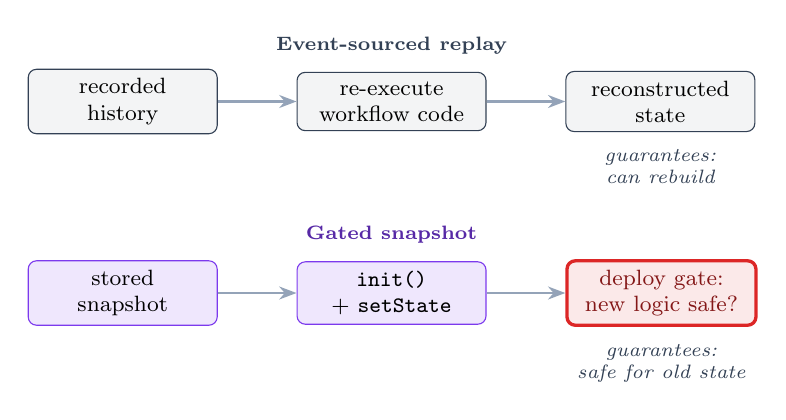
\begin{tikzpicture}[font=\footnotesize, node distance=6mm]
% replay panel
\node[rectangle, rounded corners=3pt, draw=cInk, fill=cInk!6, align=center, minimum width=24mm] (hist) {recorded\\ history};
\node[rectangle, rounded corners=3pt, draw=cInk, fill=cInk!6, right=10mm of hist, align=center, minimum width=24mm] (reexec) {re-execute\\ workflow code};
\node[rectangle, rounded corners=3pt, draw=cInk, fill=cInk!6, right=10mm of reexec, align=center, minimum width=24mm] (rebuilt) {reconstructed\\ state};
\draw[flow] (hist) -- (reexec); \draw[flow] (reexec) -- (rebuilt);
\node[font=\scriptsize\bfseries, text=cInk, above=1mm of reexec] {Event-sourced replay};
\node[font=\scriptsize\itshape, text=cInk, below=1mm of rebuilt.south, align=center, anchor=north] {guarantees:\\ can rebuild};
% snapshot panel
\node[rectangle, rounded corners=3pt, draw=cVers, fill=cVers!12, align=center, minimum width=24mm, below=16mm of hist] (snap) {stored\\ snapshot};
\node[rectangle, rounded corners=3pt, draw=cVers, fill=cVers!12, right=10mm of snap, align=center, minimum width=24mm] (set) {\code{init()}\\ + \code{setState}};
\node[rectangle, rounded corners=3pt, draw=cGate, very thick, fill=cGate!10, text=cGate!60!black, right=10mm of set, align=center, minimum width=24mm] (gate) {deploy gate:\\ new logic safe?};
\draw[flow] (snap) -- (set); \draw[flow] (set) -- (gate);
\node[font=\scriptsize\bfseries, text=cVers!70!black, above=1mm of set] {Gated snapshot};
\node[font=\scriptsize\itshape, text=cInk, below=1mm of gate.south, align=center, anchor=north] {guarantees:\\ safe for old state};
\end{tikzpicture}
\caption{Two answers to ``what happens to in-flight state when the logic
changes.'' Replay guarantees that old state can be reconstructed; the gated
snapshot approach checks that the new logic is safe for the old state, which is a
different and stronger guarantee, at the cost of forcing the compatibility
question at deploy time.}
\label{fig:replay}
\end{figure}

\subsection{Which approach suits which domain}

The two approaches are not universally ranked; they fit different domains.
Replay is an audit mechanism first and a versioning mechanism second, and it
suits domains where the past must be litigated: banking, and compliance regimes
that must reproduce the exact decision procedure of some earlier date. Where the
governing requirement is ``prove what the system did,'' event sourcing holds a
card the snapshot model concedes, and Section 5 already granted it. The gated
snapshot approach suits domains where the governing requirement is ``prove the
change is safe for what is running now,'' and where the state space evolves
quickly enough that a permanent determinism tax on every change is a serious
drag. It is worth noting that the domains usually invoked as the most
safety-critical, such as flight control, are precisely the ones that already
write invariants and model-check, and that never adopted replay for anything but
telemetry forensics. The snapshot-plus-gates approach earns the audit trail back
piecewise, as Section 5 described, through per-step version stamping, explicit
migration records, and a version-aware audit, which covers most of what a
compliance regime actually asks for without paying the determinism tax on every
future change.

\section{Why this is a better way to build and maintain stateful code with agents}

The case for the lifecycle over review alone rests on five points, and they
compound.

First, it catches the defects that testing structurally cannot. A test suite
checks the situations someone thought to write down. The exhaustive exploration
checks every situation the machine can reach over the declared domain. The
double charge, the refund after ship, the stuck order live in combinations
nobody enumerated, and that is exactly what the exploration walks.

Second, the expensive part is now cheap. The reason exhaustive checking never
went mainstream was not that the mathematics is hard but that building the
harness, capturing honest ground truth, and writing the specifications was
months of labor. That labor is precisely what an agent supplies, which is why a
verification-gated lifecycle is newly practical rather than merely desirable.

Third, it changes deployment from a discipline into a gate. Because durability
is snapshot-based and each deployment is gated on the live fleet, the team stops
maintaining determinism sandboxes and stops keeping old code paths alive
indefinitely. The machine may be rewritten freely, and the gate reports whether
the rewrite is safe for the state in production.

Fourth, it never rewards a false sense of safety. Every gate exits with a
failing signal when it verified less than it appears to: a bounded exploration
that ran out of budget, an empty invariant set, a corpus with no windows, a thin
invariant set with a low mutation grade. The failure mode of verification
tooling is not a wrong answer but a reassuring one, a green result for a run that
checked almost nothing, and the entire toolset is built so that reassurance must
be earned. That this danger is real and not hypothetical has recent empirical
support: TLA-Prover reports that model-generated specifications routinely pass
the TLC model checker while being mutation-insensitive, that is, vacuous, and
that untuned generation produces such specifications at a measurable
rate~\cite{tlaprover}. A green model check is therefore not, on its own, evidence
of anything, which is precisely why every gate here discloses the strength of
what it checked rather than only whether it passed.

Fifth, it puts human effort where it is decisive and removes it from where it is
not. The agent drafts, writes, tests, triages, and repairs. The human decides
what the software is and what it must never do, and both decisions take minutes.
The result is that a team maintains stateful code by maintaining its intent, and
the code is regenerated or repaired to match, rather than by reviewing every
line an agent produced.

\section{Threats to validity}

The honest ledger has several columns. The foundational experiments are
exploratory and preliminary: one task family, one model family in the body of
the studies, and five generations per cell, which support signature-level
observations but not effect-size estimates. The word ``exhaustive'' throughout
means exhaustive over the declared finite domains of the SAM v2 strict profile,
not over arbitrary state machines; the gap between a declared domain and the
values production actually carries is unmeasured human judgment, and the reports
say so. That phrasing needs one correction, which a replication on an external
benchmark task forced. \emph{Finite action domains do not imply a finite state
space.} On the etcd Raft task the declared domains are finite and small, and the
reachable space is nonetheless unbounded, because an election timeout increments
a term that no contract field bounds: the state accumulates across steps rather
than being drawn from a domain. Exploration on such a machine terminates at the
cap for every specification at every budget, so a clean exhaustive verdict is
not merely expensive there, it is unreachable, and the only verdicts available
are a definitive violation or an inconclusive bounded run. Exhaustiveness
therefore requires a finite \emph{reachable state space}, which is strictly
stronger than finite action domains and is a condition a contract is not
currently required to declare. Machines with an accumulating unbounded field --
a counter, a sequence number, a term -- all have this property. Every compatibility guarantee is relative to the invariants a human
stated, so intent that the invariants do not mention is invisible to every gate,
and the checker is safety-oriented, so a version that silently stops doing
something a safety invariant never required will pass. The single most important
bound, that every guarantee is relative to the observable-state projection, is
stated as a first-class limitation in Section~\ref{sub:projection} rather than buried here,
because it is the ceiling on the whole approach, and the cross-machine product
gap of Section~\ref{sub:product} is the same limitation showing its edge rather than a separate
item. Three further boundaries answer questions a practitioner will ask.
External state dependencies, such as a billing system the machine talks to, are
outside the model; the toolset checks the machine, not its dependencies, and
assumes they are versioned separately, with their outcomes entering the machine
only as declared input domains. Nondeterministic and eventually-consistent
external outcomes are handled the same way, as the open-world input space: the
explorer delivers every declared payload in every reachable state, including
outcomes a correct external system would not produce, so the machine must be
robust to all of them, but the check does not simulate wall-clock timing or
consistency windows, only the space of outcomes as inputs. Deployment velocity is
a real constraint, because a gate that takes hours will be bypassed; the gates
are deterministic, require no model at inference time, and seed from the small set
of distinct observable states rather than from the raw fleet, which keeps them
CI-fast for typical machines, with the honest caveat that a large declared domain
can push a run toward the bounded verdict and longer times, which is exactly the
completeness-threshold question Section~\ref{sub:seeded} names. The fleet study of Section~\ref{sub:fleetstudy} carries its own
column, and it is the one a reader should weigh hardest, because it is the only
place the paper reports operational numbers. Its corpora are generated by the
models under study rather than captured from running systems. For the
compatibility question actually asked, whether states the old version declares
legal remain legal under the new one, a model-generated corpus is the right
input and the study's over-approximating abstractions make it, if anything,
harsher than a live fleet would be. But it is circular as evidence about the
models themselves, which is why the harness refuses to compute true-positive and
false-positive rates over the generated subscription corpus at all, and why that
adjudication waits on a live capture rather than being estimated. In the
archaeology tier the ground truth is external, drawn from the maintainers'
migrations and their own account of the change, but the \emph{models} are ours:
two hand translations of somebody else's code, and whoever writes such a
translation controls which findings are expressible. The freeze protocol answers
that as directly as we know how, by committing each old-version model before the
new version's diff is read, so a finding cannot encode an answer already known;
the freeze commits are cited with the results. It does not eliminate the
concern. The tier covers two version pairs of one project in one subsystem, and
it produced no true positive in the strict sense, because the project shipped no
change in that window whose migration a finding could name. Finally, the author
is the author of the SAM pattern, so the revision study confirms enforcement on
the exact failure classes it was designed against rather than demonstrating that
the enforcement generalizes; an independent replication on a different task
remains the right next test, now alongside a live-fleet capture and a wider
archaeology sample. None of these are reasons to distrust the construction, but
all of them bound what it claims.

\section{Conclusion}

The trust question that coding agents raise for stateful code does not have a
review-shaped answer, because no reviewer can enumerate the reachable states
that hide the defects. It has a gate-shaped answer. The \tool{polygraph}
toolset supplies the gates: it makes the observable state a sealed declaration
so that shape compatibility is a mechanical round-trip over the live fleet, it
makes semantics checkable so that ``can the new rules hurt old state'' is a
model check seeded from production snapshots rather than a review judgment, it
makes in-flight stimuli safe by the same verified rejection that makes
redelivery safe, it makes vocabulary drift a load-time error, it makes
migration a pure and gated and fenced and journaled artifact, and it elicits
and grades the invariants on which every other gate depends. The genesis of the
toolset in the SysMoBench experiments is what gives these choices their
warrant, because those experiments established that contract shape is a real
lever and produced the strict profile that makes the obligations checkable.
\tool{polyvers} is the part we believe is genuinely new: it defines
compatibility as a computable property over the states the fleet actually
holds, and mechanizes the landmine hunt that every long-running workflow system
faces and few name. The fleet study turns that claim from an argument into a
controlled result: the same tool passes or fails the same change on nothing but
corpus provenance, an archived corpus catching a landmine a synthesized one
cannot, and the one finding the study missed lands exactly on the projection
ceiling, a declared money abstraction that collapses at zero, which is the honest
limit made measurable rather than conceded in the abstract. Versioning stateful
code stops being a permanent discipline
practiced on every change and becomes a set of gates a change either passes or
fails, with the standing and openly stated caveat that the gates are exactly as
good as the invariants a human bothered to state.

\appendix

\section*{Glossary}
\addcontentsline{toc}{section}{Glossary}

\begin{description}[leftmargin=0pt, style=nextline]
\item[State machine] Software that occupies one of several defined situations
  (states) and moves between them on events. Most business software is a state
  machine whether or not it is drawn as one.
\item[State] The current situation of one instance, together with the data that
  accompanies it (an amount, an address). An order in \emph{shipped} is a state.
\item[Fleet] All the live instances of a machine running in production at a
  given moment, taken together. Changing the code changes something on which
  thousands of in-progress instances depend.
\item[Invariant] A property that must hold in every reachable state, no matter
  what sequence of events arrives (``a customer is never charged twice''). The
  invariants are the ``must never happen'' list a human owns.
\item[Contract] The declared description of a machine: which observable state
  keys exist, which actions are allowed, what data they carry, which states are
  terminal. Everything downstream is checked against it.
\item[Observable state] The fields that constitute a machine's situation, as
  opposed to incidental bookkeeping. Choosing it is a modeling decision no tool
  can make.
\item[Model checking] Automatically exploring every situation a machine can
  reach and confirming the invariants hold in all of them, or producing the one
  situation that breaks them. Exhaustive where testing samples.
\item[Bounded model checking] Model checking limited to a finite region, here
  the declared finite domains of actions and payloads and an exploration cap. A
  bounded run that hits the cap is reported as bounded, never as a clean pass.
\item[Reachable state] Any situation a machine can actually reach by some
  sequence of real events. Defects hide in the reachable states nobody expected
  to be reachable.
\item[Counterexample] When a rule can be broken, the shortest sequence of steps
  that breaks it: a ready-made bug reproduction rather than a vague warning.
\item[SAM pattern] State-Action-Model, a state-machine pattern whose
  decomposition into actions, acceptors, and a model mirrors the action
  semantics of TLA+. The common substrate of the toolset.
\item[Action] In SAM, the part that computes a proposed change (a proposal)
  from an input.
\item[Acceptor] In SAM, the part that guards a proposal against the current
  model and either applies it or rejects it. The sole locus of mutation.
\item[Reject (observable rejection)] A first-class, named no-op returned when an
  action does not apply in the current state, so that ``this did not apply'' is
  a visible, classifiable event rather than silence.
\item[Bare-next contract] The minimal alternative to SAM: a single pure
  transition function \code{next(state, action, data)} with no framework. Faithful
  for replay, but not mechanically checkable.
\item[SAM v2 strict profile] The revised SAM library that turns five documented
  failure classes (silent no-op wiring, hidden state, silent rejection,
  dispatching monolith, undeclared domain) into construction-time or first-fire
  errors.
\item[Window] A unit of ground truth of the form (pre-state, action, data,
  post-state) captured from code executing. The universal currency all engines
  share.
\item[Trace] A sequence of windows captured from a real execution, stored as
  newline-delimited JSON. Used to check a specification against reality.
\item[Replay] Running captured windows through a specification and comparing its
  output to what actually happened. Finds unfaithfulness, not bugs.
\item[Snapshot] The stored observable state of one instance, used to rehydrate
  it without replaying its history.
\item[Durable execution] Running long-lived processes so they survive crashes,
  restarts, and deployments without losing their place.
\item[Seeded model check] The \tool{polyvers} technique of adding live fleet
  snapshots as additional starting points of an exhaustive exploration, to ask
  whether any state production currently holds can be driven to a violation
  under new rules.
\item[Lane] In \tool{polyvers}, a category of change (shape, semantic,
  vocabulary, intent, migration, composition) that a difference of the artifact
  family fires, each demanding specific gates.
\item[Migration] A pure function from old state to new state, used when the
  shape changes. Validated across the whole fleet before any instance is
  altered.
\item[Effect mapper] The pure mapping from transitions to external effects (send
  an email, charge a card), checked for emission invariants before deployment.
\item[Mutation testing] Assessing the strength of a set of checks by
  deliberately introducing small defects and seeing whether the checks catch
  them. Used by \tool{polynv} to grade invariant sets.
\item[Transpiler] Here, the tool that mechanically translates a structured SAM
  specification into a TLA+ model that a model checker evaluates. Possible for
  SAM, impossible for the bare-next contract.
\item[TLA+ / TLC] A formal specification language for concurrent and
  distributed systems, and its model checker.
\item[Poison] In \tool{polyrun}, the state an instance is durably moved to when
  something that ``cannot happen'' for a verified machine happens: a loud defect
  alarm rather than silent corruption.
\end{description}

\begin{thebibliography}{99}

\bibitem{jsam2} J.-J.\ Dubray. \emph{Executable JavaScript as a Checkable
Specification Language: A JS-SAM Case Study on SysMoBench.} Manuscript,
arXiv:2607.05076, 2026.

\bibitem{jsam1} J.-J.\ Dubray. \emph{Executable JavaScript as a Checkable
Specification Language: Agent-Mediated TLA+ Phase 3, the Etcd Raft Study, and
Repair Rounds.} Manuscript, arXiv:2607.13092, 2026.

\bibitem{robust} J.-J.\ Dubray. \emph{Formal Structure in LLM-Written
Specifications: Separating Robustness from Verifiability.} Manuscript, 2026.

\bibitem{sam} J.-J.\ Dubray. \emph{The SAM Pattern.} \url{https://sam.js.org},
2016 onward.

\bibitem{samv2} J.-J.\ Dubray. \emph{sam-pattern v2 strict profile} (package
\texttt{@cognitive-fab/sam-pattern}, v2.0.0-alpha.1).
\url{https://github.com/jdubray/sam-lib/tree/v2}, 2026.

\bibitem{repo} J.-J.\ Dubray. \emph{Polygraph toolset and fleet-study artifacts}
(pre-registration, taxonomy, run harness, and freeze commits under
\texttt{eval/fleet-study/}). \url{https://github.com/jdubray/polygraph}, 2026.

\bibitem{sysmobench} Specula. \emph{SysMoBench: Benchmarking AI on Formally
Modeling Complex Real-World Systems.} \url{https://sysmobench.com}, 2026.

\bibitem{lamport} L.\ Lamport. \emph{Specifying Systems: The TLA+ Language and
Tools for Hardware and Software Engineers.} Addison-Wesley, 2002.

\bibitem{daikon} M.\ D.\ Ernst et al. \emph{The Daikon System for Dynamic
Detection of Likely Invariants.} Science of Computer Programming, 2007.

\bibitem{vanlamsweerde} A.\ van Lamsweerde and L.\ Willemet. \emph{Inferring
Declarative Requirements Specifications from Operational Scenarios.} IEEE
Transactions on Software Engineering, 1998.

\bibitem{oracle} G.\ Fraser and A.\ Zeller. \emph{Test Oracle Assessment and
Improvement} (mutation-based oracle strength). Proc. ISSTA, 2012.

\bibitem{specfuzzer} F.\ Molina et al. \emph{Specification Fuzzing: Generating
Assertions with Grammar-Based Fuzzing, Dynamic Invariant Detection, and
Mutation Analysis (SpecFuzzer).} Proc. ASE, 2021.

\bibitem{subtyping} R.\ H.\ Reussner et al. \emph{Checking Behavioural Subtypes
via Refinement (FDR/CSP).} 2003.

\bibitem{session} J.\ Lange and N.\ Yoshida. \emph{Undecidability of
Asynchronous Session Subtyping.} Logical Methods in Computer Science, 2017.

\bibitem{dsu} C.\ M.\ Hayden, E.\ K.\ Smith, M.\ Hicks, and J.\ S.\ Foster.
\emph{Specifying and Verifying the Correctness of Dynamic Software Updates.}
Proc. VSTTE, 2012.

\bibitem{temporalwv} Temporal Technologies. \emph{Worker Versioning} (Build IDs,
Pinned and Auto-Upgrade behaviors, Upgrade on Continue-as-New).
\url{https://docs.temporal.io/production-deployment/worker-deployments/worker-versioning},
2025.

\bibitem{upcasting} K.\ Overeem, M.\ Spoor, and S.\ Jansen. \emph{The Dark Side
of Event Sourcing: Managing Data Conversion.} Proc. SANER, 2017. (Schema
evolution and upcasting in event-sourced systems.)

\bibitem{restate} Restate. \emph{Building a Modern Durable Execution Engine from
First Principles} (journal-based durable execution).
\url{https://www.restate.dev}, 2025.

\bibitem{dbos} DBOS. \emph{Durable Execution as a Library: Postgres-Backed
Workflow and Step Checkpointing.} \url{https://www.dbos.dev}, 2025.

\bibitem{directed} S.\ Edelkamp, S.\ Leue, and A.\ Lluch-Lafuente. \emph{Directed
Explicit-State Model Checking in the Validation of Communication Protocols.}
International Journal on Software Tools for Technology Transfer, 2004.

\bibitem{tlaprover} E.\ Spencer, A.\ Bisharat, B.\ Ortiz, K.\ Bhadauria, T.\
Wang, G.\ K.\ Thiruvathukal, K.\ L\"aufer, and M.\ Abuhamad. \emph{TLA-Prover:
Verifiable TLA+ Specification Synthesis via Preference-Optimized Low-Rank
Adaptation.} arXiv:2606.06133, 2026.

\end{thebibliography}

\end{document}
